

%\begin{figure*}[htbp!]
%\centering
%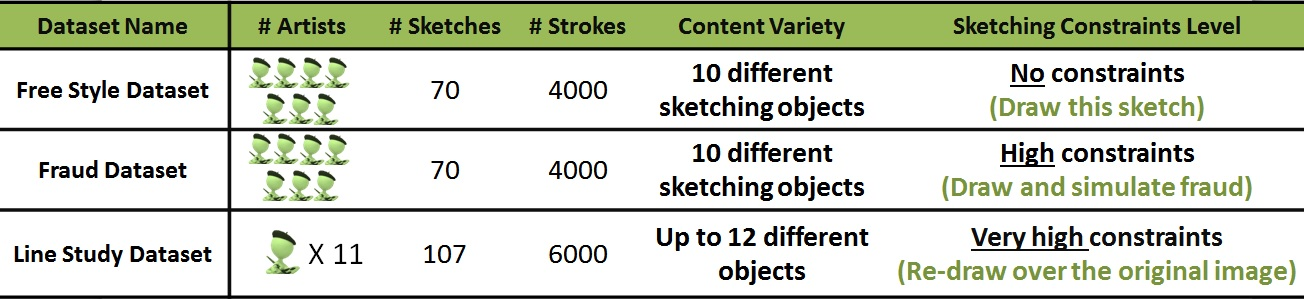
\includegraphics[width = 0.95\textwidth]{images/compDatasets.jpg}
%\vspace{-1mm}\caption {A summary of datasets used in this paper. We compiled the first two and reused the line study dataset of %~\protect\cite{Cole:2008:PDL:1360612.1360687}.}\vspace{-5mm}
%\label{datasetSummary}
%\end{figure*}


\begin{table*}[htbp!]
\begin{tabular}{|c|ccccc|}
\hline
\textbf{Dataset}                          & \textbf{\# Artists} & \textbf{\# Sketches} & \textbf{\# Strokes} & \textbf{Content Variety}       & \textbf{Sketching Constraints Level}                                                              \\ \hline
\textbf{Free Style}                       & 7                   & 70                   & 4000                & 10 different sketching objects & \begin{tabular}[c]{@{}c@{}}No constraints\\ (Draw this sketch)\end{tabular}                       \\ \hline
\textbf{Fraud}                            & 7                   & 70                   & 4000                & 10 different sketching objects & \begin{tabular}[c]{@{}c@{}}High constraints\\ (Draw and simulate fraud)\end{tabular}              \\ \hline
\multicolumn{1}{|l|}{\textbf{Line Study}} & 11                  & 107                  & 6000                & Up to 12 different objects     & \begin{tabular}[c]{@{}c@{}}Very high constraints\\ (Re-draw over the original Image)\end{tabular} \\ \hline
\end{tabular}
\vspace{-1mm}\caption {A summary of datasets used in this paper. We compiled the first two and reused the line study dataset of ~\protect\cite{Cole:2008:PDL:1360612.1360687}.}\vspace{-4mm}
\label{datasetSummary}
\end{table*}

%(e.g. the same object, the same object from different views, and different objects are sketched multiple times)
To evaluate the performance of SAR, we compile two new sketch datasets collected from experienced artists. Participating artists were screened, so as to guarantee high levels of sketching capability. The chosen artists were graphical or interior designers by profession, each with 7-10 years of sketching experience. We gave them the freedom to draw using a pen, pencil or digitally at any scale. Moreover, they were allowed to correct their strokes or redraw the entire sketch with no time limit. Since we had direct access to these professionals, we were able to administer different sketching scenarios. This allowed us to control the \emph{content variety} (i.e. what the artist draws in a sketch) and the extent of \emph{sketching constraints} (i.e. how the artist should sketch). These two factors impact the strokes an artist chooses and ultimately his/her style. To our knowledge, this work is the first to compile such a diverse set of sketch data for the purpose of studying authorship from strokes. To allow for further research in this area, we will make all these datasets (images and annotations) publicly available. Next, we describe the datasets used in this paper (refer to Table \ref{datasetSummary} for a summary).


%there does not exist an available dataset of sketches such that the same set of sketches are drawn by multiple artists who are either freely drawing without constraints or attempting to make their sketches as close as possible to the original set of sketches. With the help of a number of valued artists, we collected sketches of 3 different datasets. Participating artists have demonstrated a high level of sketching abilities through their work as some of them are graphical designers and others are interior designers and they have an average sketching experience of 7 years and a maximum of 10 years. These datasets are created such that SAR is  exposed incrementally to 3  different levels of difficulties and challenges as will be discussed in details in the following sections. We made all the sketches available as part of contribution provided in this work and we hope that interesting studies can be applied using them.
%\vspace{-2mm}
%\paragraph{Flower Dataset.} In this dataset, four different artists were provided an image of a simple flower sketch and asked to draw it multiple times as they see fit. In this case, the same object is being sketched multiple times (i.e. the content variety is minimal). Moreover, artists were given complete freedom to draw the assigned sketch without any constraints or specific instructions. We will see that this constraint-free type of sketching allows artistic style to be more distinguishable among different artists than constraint-ridden sketching, of which sketch fraud is a prime example. This dataset will be the first test of SAR's ability to determine authorship from sketched strokes alone.

%constrained sketching tasks and thus experimenting using this dataset is considered to be the first milestone to test the performance of SAR.
%\vspace{-2mm}
%\paragraph{Character Dataset.} Unlike the previous dataset, artists in this dataset were asked to sketch the same cartoon character viewed from 12 distinct viewpoints. We chose Mickey Mouse, a famous Disney character, because it is a well known character and relatively easy to sketch. Artists were encouraged to draw as close as possible to the cartoon images given to them and no further instructions were given. This dataset clearly presents a higher level of challenge as compared to the flower dataset, especially since content variety here is significantly higher.

%Using this dataset, SAR is exposed to a higher level of challenge compared to the previous flower sketches because as the level of sketching constraints assigned is slightly higher and there is more content variety. i.e. we attempt to identify the authorship of a sketch by comparing it to a different content.

%We first collected the different views of Mickey images over the web and we asked 3 different artists to sketch them.

%\vspace{-2mm}
\noindent\textbf{Free Style Dataset.} We collected 10 images of objects from diverse semantic categories and then asked 7 artists to sketch them. The objects were chosen to be detailed enough to adequately reflect artistic style and to be relatively easy to replicate by an experienced artist in a reasonable amount of time. The 70 sketches (10 from each artist) were collected in three weeks. No constraints or specific instructions were given to the artists, thus, giving them complete sketching freedom.
%We will see that this constraint-free type of sketching allows artistic style to be more distinguishable among different artists than constraint-ridden sketching, of which sketch fraud is a prime example. %This dataset will be the first test of SAR's ability to determine authorship from sketched strokes alone.


%\vspace{-2mm}
\noindent\textbf{Fraud Dataset.}  Here, we simulate a sketch fraud scenario. Using the same images in the free style dataset, we chose the sketches of one of the artists as \emph{original} drawings. We asked the other 6 artists to draw all the original sketches. We provided them with an instruction sheet, where they were requested to draw the original sketches in such a way that it would be very hard to distinguish their \emph{own} drawings from the originals, thus, simulating sketch fraud. The 6 artists were prohibited from using methods or supplies (e.g. translucent tracing paper) that could produce copies of the original sketches. Over a period of 2 weeks, we collected a total of 60 sketches. (refer to Figure \ref{FraudDataset} for examples). Since the artists were requested to simulate sketch fraud, this dataset is highly constrained from an artistic style perspective. Therefore, it poses a substantial challenge to any authorship recognition system, albeit manual or automatic.

%\begin{figure*}[htbp!]
%\centering
%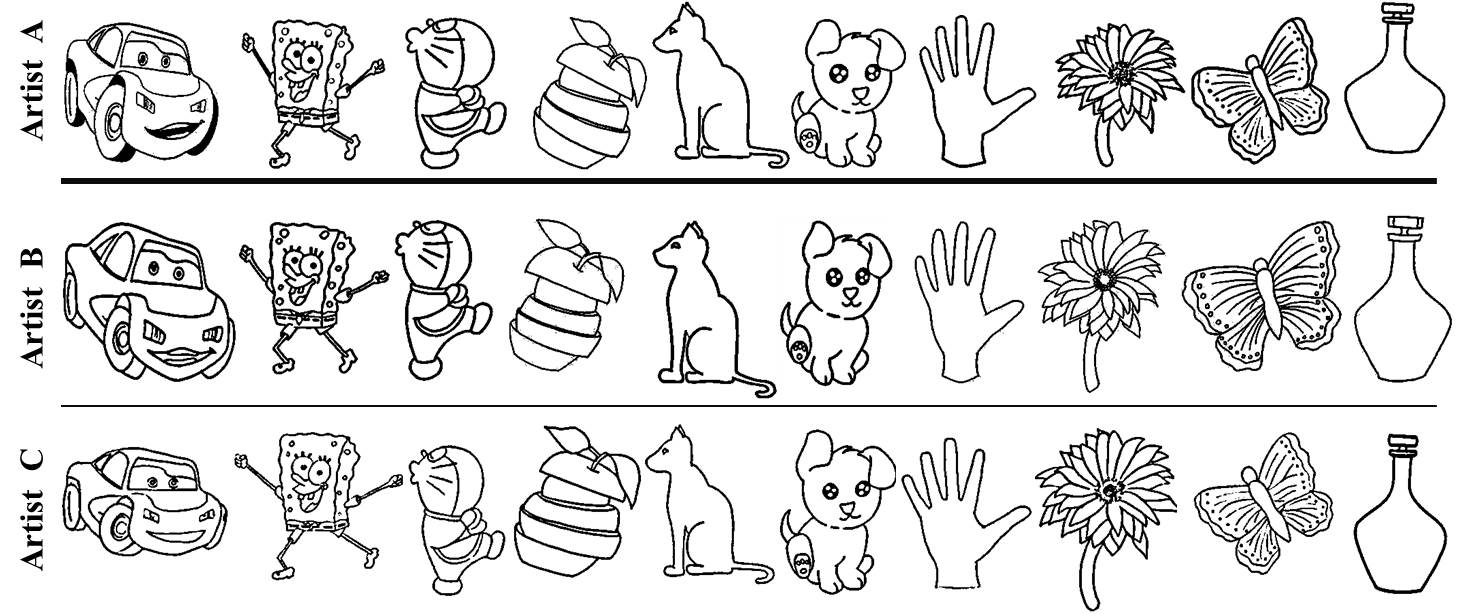
\includegraphics[width = 1.0\textwidth]{images/fraudExperiment.jpg}
%\vspace{-6mm}\caption {Samples of sketches from the fraud dataset. The first row shows the original sketches drawn by Artist A. The other three rows show the sketches of 2 other artists (Artists B and C), who attempted  sketch fraud. Obviously, the \emph{fraudulent} sketches look extremely similar to the originals, making authorship recognition (manual or automatic) quite difficult.}\vspace{-5mm}
%\label{FraudDataset}
%\end{figure*}

%In this dataset, we simulate a sketch fraud scenario. We first collected 10 objects of various semantic categories and asked one of the participating artists to sketch them. From a fraud perspective, these 10 sketches can be considered to be \emph{original} drawings. The objects were chosen to be detailed enough to adequately reflect the artists' sketching style and to be relatively easy for any experienced artist to replicate in a reasonable amount of time. After the originals were generated, we tasked 6 other artists to draw them. Along with the original sketches, we provided them with an instruction sheet, in which we asked them to draw the provided sketches such that it would be very hard to distinguish their \emph{own} drawings from the \emph{original} ones, thus, simulating sketch fraud. The 6 artists were prohibited from using methods or supplies (e.g. translucent tracing paper) that would enable them to produce copies of the original sketches. Over a period of 2 weeks, we collected a total of 70 sketches from the 7 artists. Some sample sketches are shown in Figure \ref{FraudDataset}. Since the artists were requested to simulate sketch fraud, the generated dataset is considered highly constrained and significantly diverse in content. It poses a substantial challenge to any authorship recognition system, albeit manual or automatic.


%compiled a fraud experiment which we conducted with the aim to experiment SAR on a variety of datasets types and to expose our techniques to different levels of challenges to assess its effectiveness and value. In our experiment, we first collected 10 subjects under various categories to be sketched initially by one of the collaborating artists in our experiment.

%The subjects are chosen such that they are detailed enough to adequately reflect the artist's sketching style under different sketching subjects and to be considerably easy for any artist to replicate and not time consuming as well.

%In the next stage of the experiment, we assigned 6 other artists to draw the sketches provided by the first artist. Along with the sketches, we provided them with an instruction sheet in which we asked them to sketch the assigned sketches such that it is hard to distinguish their drawings from the original ones so that they simulate a sketching fraud attempt.

%Moreover, they were allowed to correct their strokes or redraw the entire sketch if they needed we assigned no time limit for them to draw.

%Artists, on the other hand, were encouraged to use strong, dark and smooth lines, be especially accurate to make the sketches very similar to the presented sketches and were prohibited to copy the sketches.

%Towards the end of the experiment which expanded for a period of 2 weeks, we collected a total of 70 sketches provided by 7 artists. A sample of these sketches is in figure ~\ref{FraudDataset}.

%Given that artists were requested to simulate a fraud attempt while sketching the assigned subjects, we consider the sketching task for this dataset to be highly constrained and thus more challenging to SAR than the previous 2 datasets.




%\vspace{-2mm}
\noindent\textbf{Line Study Dataset.} We also use the line study dataset generated in \cite{Cole:2008:PDL:1360612.1360687}. This dataset is a collection of sketches of various objects (e.g. mechanical tools, automobile parts, and bones) drawn by multiple artists. The sketching tasks were highly constrained, since artists were asked to draw their sketched lines over a faded copy of the original image. Clearly, the task of recognizing sketch authorship in this dataset is more difficult than the previous two. We selected all sketches from artists, who drew at least 6 sketches, thus, leading to a dataset of 107 sketches from 11 artists.  %Given such highly constrained sketching tasks, we want to experiment the performance of SAR and compare this against.
%{\color{red} [Put a reference next to the Line Study dataset]}

%Figure ~\ref{datasetSummary} provides a summary of all the datasets described above.
